% Native editable composition from verified, unchanged IDE images.
\begin{figure}[htbp]
\centering
\sbox0{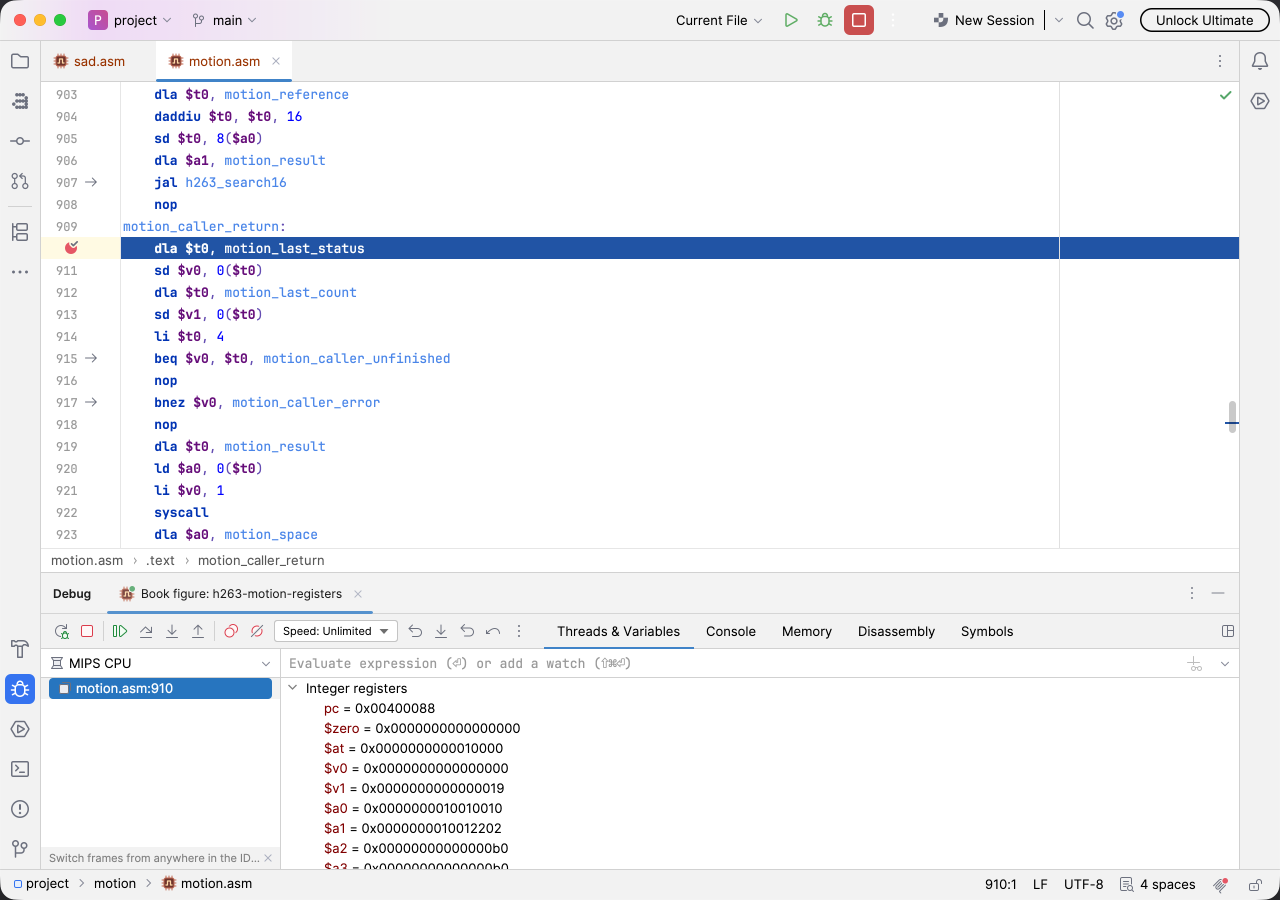
\includegraphics[artifact]{book/captures/035-h263/h263-motion-result/registers.png}}
\sbox2{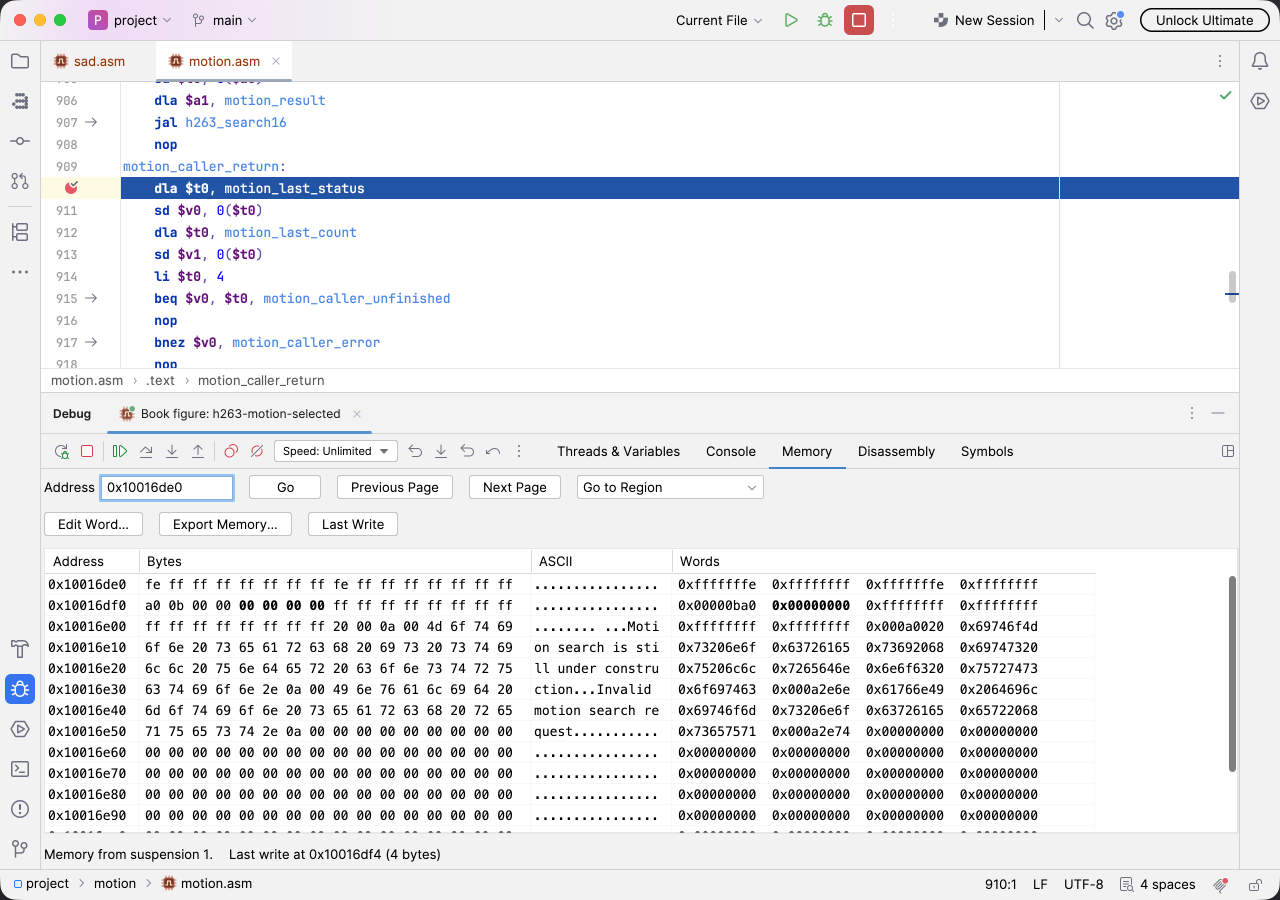
\includegraphics[artifact]{book/captures/035-h263/h263-motion-result/selected.png}}
\edef\MARSmotionsourceLeft{\the\dimexpr0.036718750\wd0\relax}
\edef\MARSmotionsourceBottom{\the\dimexpr0.707777778\ht0\relax}
\edef\MARSmotionsourceRight{\the\dimexpr0.611718750\wd0\relax}
\edef\MARSmotionsourceTop{\the\dimexpr0.236666667\ht0\relax}
\edef\MARSmotionselectedLeft{\the\dimexpr0.520312500\wd2\relax}
\edef\MARSmotionselectedBottom{\the\dimexpr0.312222222\ht2\relax}
\edef\MARSmotionselectedRight{\the\dimexpr0.139843750\wd2\relax}
\edef\MARSmotionselectedTop{\the\dimexpr0.634444444\ht2\relax}
\edef\MARSmotionreturnsLeft{\the\dimexpr0.246093750\wd0\relax}
\edef\MARSmotionreturnsBottom{\the\dimexpr0.110000000\ht0\relax}
\edef\MARSmotionreturnsRight{\the\dimexpr0.596875000\wd0\relax}
\edef\MARSmotionreturnsTop{\the\dimexpr0.838888889\ht0\relax}
\begin{tikzpicture}[alt={Three annotated IDE details at motion_caller_return. The next instruction forms the saved-status address. The native Words view shows little-endian low/high pairs for dx minus two, dy minus two and cost hexadecimal ba0, decimal 2976. Its final pair lies after the result record. Register v0 is zero and v1 is hexadecimal 19, decimal 25 unique admitted candidates.}]
\node[anchor=north west,inner sep=0,font=\small\bfseries] (source-title) at (6mm,0) {The search has returned};
\node[anchor=north west,inner sep=0] (source) at ([yshift=-1mm]source-title.south west) {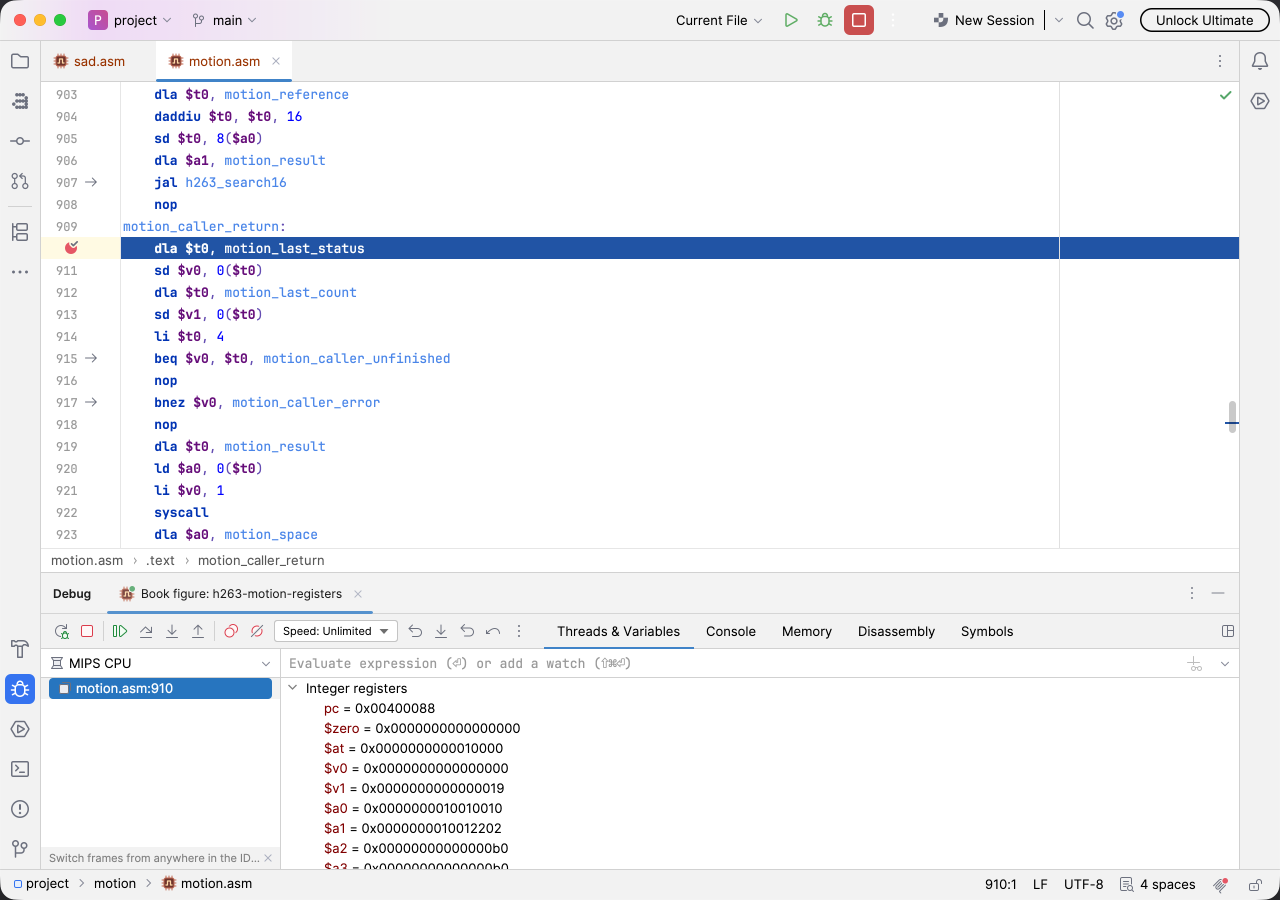
\includegraphics[width=0.7\linewidth,artifact,trim={\MARSmotionsourceLeft{} \MARSmotionsourceBottom{} \MARSmotionsourceRight{} \MARSmotionsourceTop{}},clip]{book/captures/035-h263/h263-motion-result/registers.png}};
\begin{scope}[shift={(source.south west)},x={($(source.south east)-(source.south west)$)},y={($(source.north west)-(source.south west)$)}]
\draw[black,line width=0.7pt] (0.168888889,0.080000000) rectangle (0.704444444,0.520000000);
\node[draw=black,fill=white,circle,inner sep=1.5pt,font=\footnotesize] at ($(0.168888889,0.520000000)+(-3mm,0)$) {1};
\end{scope}
\node[anchor=north west,inner sep=0,font=\small\bfseries] (selected-title) at ([yshift=-2mm]source.south west) {Three result doublewords in the Words view};
\node[anchor=north west,inner sep=0] (selected) at ([yshift=-1mm]selected-title.south west) {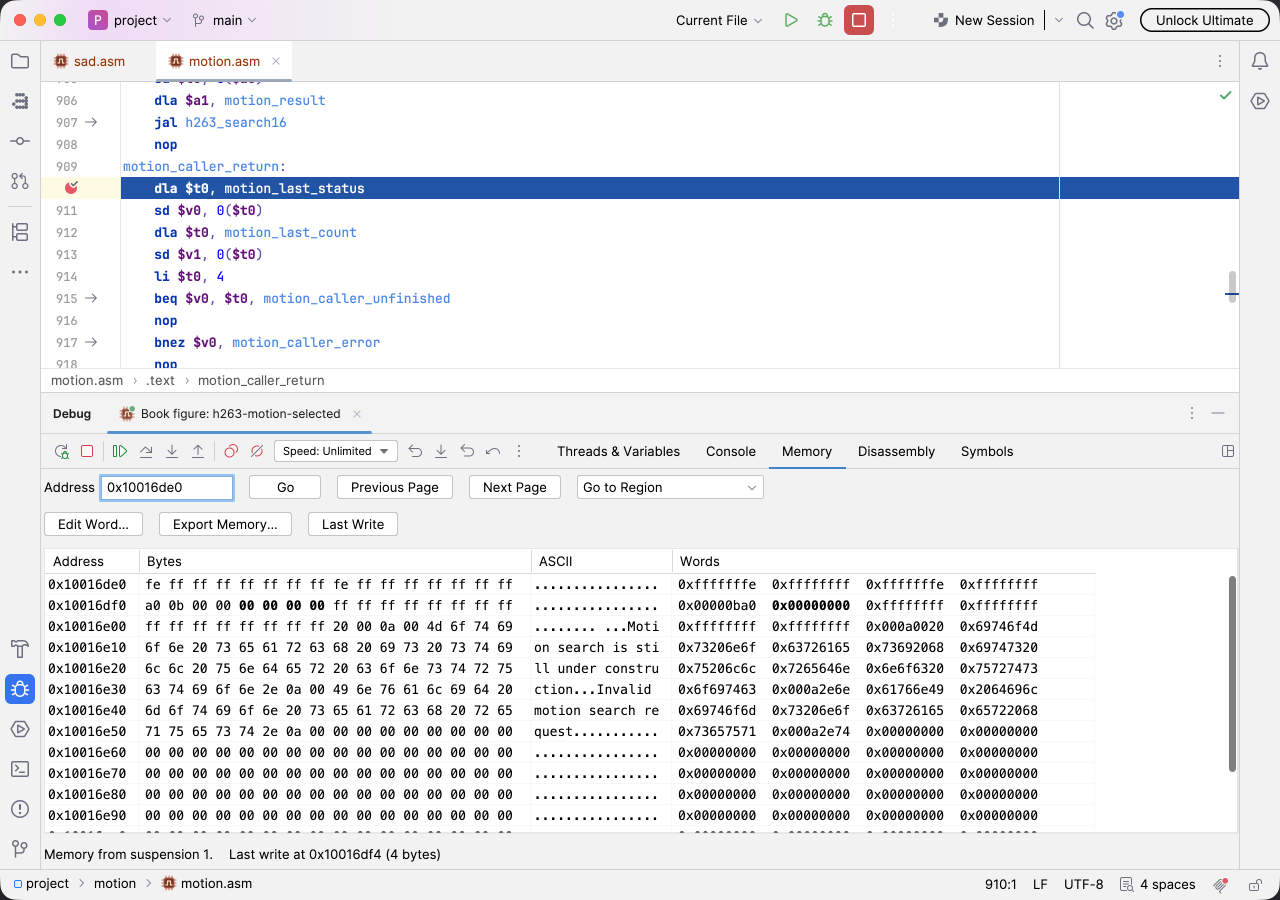
\includegraphics[width=0.84\linewidth,artifact,trim={\MARSmotionselectedLeft{} \MARSmotionselectedBottom{} \MARSmotionselectedRight{} \MARSmotionselectedTop{}},clip]{book/captures/035-h263/h263-motion-result/selected.png}};
\begin{scope}[shift={(selected.south west)},x={($(selected.south east)-(selected.south west)$)},y={($(selected.north west)-(selected.south west)$)}]
\draw[black,line width=0.7pt] (0.013793103,0.062500000) rectangle (0.986206897,0.937500000);
\node[draw=black,fill=white,circle,inner sep=1.5pt,font=\footnotesize] at ($(0.013793103,0.937500000)+(-3mm,0)$) {2};
\end{scope}
\node[anchor=north west,inner sep=0,font=\small\bfseries] (returns-title) at ([yshift=-2mm]selected.south west) {Successful search and unique candidate count};
\node[anchor=north west,inner sep=0] (returns) at ([yshift=-1mm]returns-title.south west) {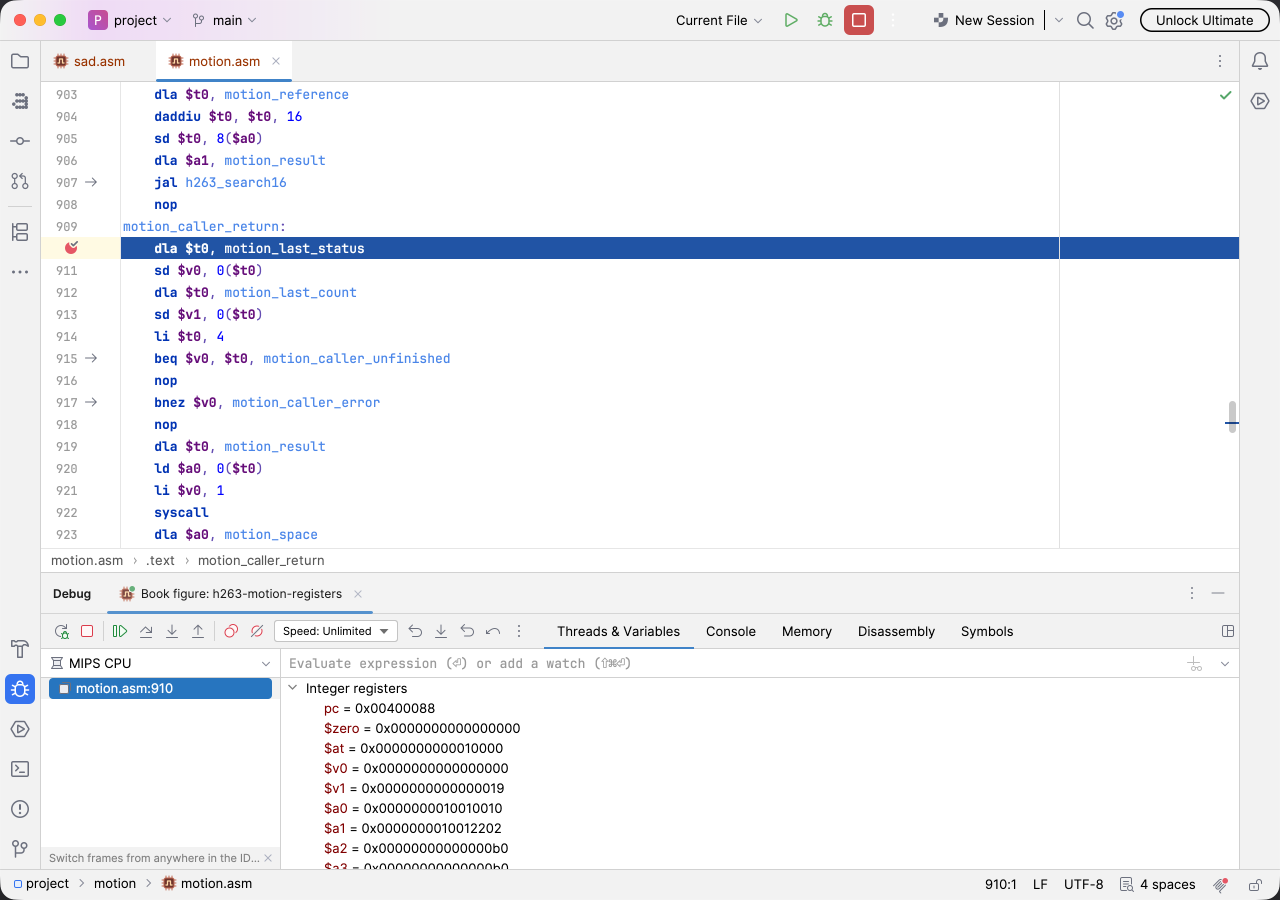
\includegraphics[width=0.5\linewidth,artifact,trim={\MARSmotionreturnsLeft{} \MARSmotionreturnsBottom{} \MARSmotionreturnsRight{} \MARSmotionreturnsTop{}},clip]{book/captures/035-h263/h263-motion-result/registers.png}};
\begin{scope}[shift={(returns.south west)},x={($(returns.south east)-(returns.south west)$)},y={($(returns.north west)-(returns.south west)$)}]
\draw[black,line width=0.7pt] (0.029850746,0.065217391) rectangle (0.970149254,0.934782609);
\node[draw=black,fill=white,circle,inner sep=1.5pt,font=\footnotesize] at ($(0.029850746,0.934782609)+(-3mm,0)$) {3};
\end{scope}
\end{tikzpicture}
\par\smallskip
\begin{minipage}{\linewidth}
\small
\begin{enumerate}
\item The search has published its result and returned. The caller has not yet copied its status and candidate count into the separate observation fields.
\item Each signed 64-bit displacement occupies two displayed 32-bit words. Read low word then high word: \texttt{fffffffe ffffffff} is $-2$ for each component. The next pair, \texttt{00000ba0 00000000}, is SAD 2976. The final two \texttt{ffffffff} words lie after the 24-byte result and retain the caller\textquoteright s old status.
\item \texttt{\$v0}=0 and \texttt{\$v1}=\texttt{0x19}=25. The count is the number of unique admitted candidates tested. It is separate from the selected candidate\textquoteright s SAD.
\end{enumerate}
\end{minipage}
\caption{The selected motion vector and its residual cost. Two Debug launches inspect the same search return.}
\label{fig:h263-motion-result}
\end{figure}
